% !TeX spellcheck = sl_SI
% vim: set spell spelllang=sl:
% za preverjanje črkovanja, če se uporablja Texstudio ali vim
\documentclass[12pt,a4paper,twoside]{article}
\usepackage[utf8]{inputenc}  % pravilno razpoznavanje unicode znakov

% NASLEDNJE UKAZE USTREZNO POPRAVI
\newcommand{\program}{Pedagoška matematika} % ime studijskega programa
\newcommand{\imeavtorja}{Simon Besednjak} % ime avtorja
\newcommand{\imementorja}{prof.~dr.~Marjetka Knez} % akademski naziv in ime mentorja, uporabi poln naziv, prof.~dr.~, doc.~dr., ali izr.~prof.~dr.
\newcommand{\imesomentorja}{} % akademski naziv in ime somentorja, če ga imate
\newcommand{\naslovdela}{Dvojne PH krivulje}
\newcommand{\letnica}{2021} % letnica magistriranja
\newcommand{\opis}{Delo obravnava lastnosti krivulj z pitagorejskih hodografom.}  % Opis dela v eni povedi. Ne sme vsebovati matematičnih simbolov v $ $.
\newcommand{\kljucnebesede}{PH krivulje\sep dvojne PH krivulje} % ključne besede, ločene z \sep, da se PDF metapodatki prav procesirajo
\newcommand{\keywords}{PH curves\sep double PH curves} % ključne besede v angleščini
\newcommand{\organization}{Univerza v Ljubljani, Fakulteta za matematiko in fiziko} % fakulteta
\newcommand{\literatura}{literatura}  % pot do datoteke z literaturo (brez .bib končnice)
\newcommand{\sep}{, }  % separator med ključnimi besedami v besedilu
% KONEC PODATKOV

\usepackage{bibentry}         % za navajanje literature v programu dela s celim imenom
\nobibliography{\literatura}
\newcommand{\plancite}[1]{\item[\cite{#1}] \bibentry{#1}} % citiranje v programu dela

\usepackage{filecontents}  % za pisanje datoteke s PDF metapodatki
\usepackage{silence} \WarningFilter{latex}{Overwriting file}  % odstrani annoying warning o obstoju datoteke
% datoteka s PDF metapodatki, zgenerira se kot magisterij.xmpdata
\begin{filecontents*}{\jobname.xmpdata}
  \Title{\naslovdela}
  \Author{\imeavtorja}
  \Keywords{\kljucnebesede}
  \Subject{matematika}
  \Org{\organization}
\end{filecontents*}

\usepackage[a-1b]{pdfx}  % zgenerira PDF v tem PDF/A-1b formatu, kot zahteva knjižnica
\hypersetup{bookmarksopen, bookmarksdepth=3, colorlinks=true,
  linkcolor=black, anchorcolor=black, citecolor=black, filecolor=black,
  menucolor=black, runcolor=black, urlcolor=black, pdfencoding=auto,
  breaklinks=true, psdextra}

\usepackage[slovene]{babel}  % slovenščina
\usepackage[T1]{fontenc}     % naprednejše kodiranje fonta
\usepackage{amsmath,amssymb,amsfonts,amsthm} % matematični paketi
\usepackage{graphicx}     % za slike
\usepackage{emptypage}    % prazne strani so neoštevilčene, ampak so štete
\usepackage{units}        % fizikalne enote kot \unit[12]{kg} s polovico nedeljivega presledka, glej primer v kodi
\usepackage{makeidx}      % za stvarno kazalo, lahko zakomentiraš, če ne rabiš
\makeindex                % za stvarno kazalo, lahko zakomentiraš, če ne rabiš
% oblika strani
\usepackage[
  top=3cm,
  bottom=3cm,
  inner=3.5cm,      % margini za dvostransko tiskanje
  outer=2.5cm,
  footskip=40pt     % pozicija številke strani
]{geometry}

% VEČ ZANIMIVIH PAKETOV
% \usepackage{array}      % več možnosti za tabele
% \usepackage[list=true,listformat=simple]{subcaption}  % več kot ena slika na figure, omogoči slika 1a, slika 1b
% \usepackage[all]{xy}    % diagrami
% \usepackage{doi}        % za clickable DOI entrye v bibliografiji
% \usepackage{enumerate}     % več možnosti za sezname

% Za barvanje source kode
% \usepackage{minted}
% \renewcommand\listingscaption{Program}

% Za pisanje psevdokode
% \usepackage{algpseudocode}  % za psevdokodo
% \usepackage{algorithm}
% \floatname{algorithm}{Algoritem}
% \renewcommand{\listalgorithmname}{Kazalo algoritmov}

% DRUGI TVOJI PAKETI:
% tukaj

\setlength{\overfullrule}{50pt} % označi predlogo vrstico
\pagestyle{plain}               % samo številka strani na dnu, nobene glave / noge

% ukazi za matematična okolja
\theoremstyle{definition} % tekst napisan pokončno
\newtheorem{definicija}{Definicija}[section]
\newtheorem{primer}[definicija]{Primer}
\newtheorem{opomba}[definicija]{Opomba}
\newtheorem{aksiom}{Aksiom}

\theoremstyle{plain} % tekst napisan poševno
\newtheorem{lema}[definicija]{Lema}
\newtheorem{izrek}[definicija]{Izrek}
\newtheorem{trditev}[definicija]{Trditev}
\newtheorem{posledica}[definicija]{Posledica}

\numberwithin{equation}{section}  % števec za enačbe zgleda kot (2.7) in se resetira v vsakem poglavju

% Matematični ukazi
\newcommand{\R}{\mathbb R}
\newcommand{\N}{\mathbb N}
\newcommand{\Z}{\mathbb Z}
\renewcommand{\C}{\mathbb C}
\newcommand{\Q}{\mathbb Q}

% \DeclareMathOperator{\tr}{tr}  % morda potrebuješ operator za sled ali kaj drugega?

% bold matematika znotraj \textbf{ }, tudi v naslovih, kot \omega spodaj
\makeatletter \g@addto@macro\bfseries{\boldmath} \makeatother

% Poimenuj kazalo slik kot ``Kazalo slik'' in ne ``Slike''
\addto\captionsslovene{
  \renewcommand{\listfigurename}{Kazalo slik}%
}

% če želiš, da se poglavja začnejo na lihih straneh zgoraj
% \let\oldsection\section
% \def\section{\cleardoublepage\oldsection}

%%%%%%%%%%%%%%%%%%%%%%%%%%%%%%%%%%%%%%%%%%
%%%%%%           DOCUMENT           %%%%%%
%%%%%%%%%%%%%%%%%%%%%%%%%%%%%%%%%%%%%%%%%%

\begin{document}

\pagenumbering{roman} % začnemo z rimskimi številkami
\thispagestyle{empty} % ampak na prvi strani ni številke

\noindent{\large
UNIVERZA V LJUBLJANI\\[1mm]
FAKULTETA ZA MATEMATIKO IN FIZIKO\\[5mm]
\program\ -- 2.~stopnja}
% ustrezno dopolni za IŠRM
\vfill

\begin{center}
  \large
  \imeavtorja\\[3mm]
  \Large
  \textbf{\MakeUppercase{\naslovdela}}\\[10mm]
  \large
  Magistrsko delo \\[1cm]
  Mentor: \imementorja \\[2mm] % ustrezno popravi spol
%   Somentor: \imesomentorja   % dodaj, če potrebno
\end{center}
\vfill

\noindent{\large Ljubljana, \letnica}

\cleardoublepage

%% sem pride IZJAVA O AVTORSTVU  -- SE NATISNE V VIS

% zahvala
\pdfbookmark[1]{Zahvala}{zahvala} %
\section*{Zahvala}
Neobvezno.
Zahvaljujem se \dots
% end zahvala -- izbriši vse med zahvala in end zahvala, če je ne rabiš

\cleardoublepage

\pdfbookmark[1]{\contentsname}{kazalo-vsebine}
\tableofcontents

% list of figures
% \cleardoublepage
% \pdfbookmark[1]{\listfigurename}{kazalo-slik}
% \listoffigures
% end list of figures

\cleardoublepage

\section*{Program dela}
\addcontentsline{toc}{section}{Program dela} % dodajmo v kazalo
Mentor naj napiše program dela skupaj z osnovno literaturo. Na literaturo se
lahko sklicuje kot~\cite{lebedev2009introduction}, \cite{gurtin1982introduction},
\cite{zienkiewicz2000finite}, \cite{STtemplate}.

\section*{Osnovna literatura}
Literatura mora biti tukaj posebej samostojno navedena (po pomembnosti) in ne
le citirana. V tem razdelku literature ne oštevilčimo po svoje, ampak uporabljamo
okolje itemize in ukaz plancite, saj je celotna literatura oštevilčena na koncu.
\begin{itemize}
  \plancite{lebedev2009introduction}
  \plancite{gurtin1982introduction}
  \plancite{zienkiewicz2000finite}
  \plancite{STtemplate}
\end{itemize}

\vspace{2cm}
\hspace*{\fill} Podpis mentorja: \phantom{prostor za podpis}

% \vspace{2cm}
% \hspace*{\fill} Podpis somentorja: \phantom{prostor za podpis}

\cleardoublepage
\pdfbookmark[1]{Povzetek}{abstract}

\begin{center}
\textbf{\naslovdela} \\[3mm]
\textsc{Povzetek} \\[2mm]
\end{center}
Tukaj napišemo povzetek vsebine. Sem sodi razlaga vsebine in ne opis tega, kako je delo
organizirano.

\vfill
\begin{center}
\textbf{English translation of the title} \\[3mm] % prevod slovenskega naslova dela
\textsc{Abstract}\\[2mm]
\end{center}

An abstract of the work is written here. This includes a short description of
the content and not the structure of your work.

\vfill\noindent
\textbf{Math.~Subj.~Class.~(2010):} oznake kot 74B05, 65N99, na voljo so na naslovu
\url{http://www.ams.org/msc/msc2010.html} \\[1mm]
\textbf{Ključne besede:} \kljucnebesede \\[1mm]
\textbf{Keywords:} \keywords

\cleardoublepage

\setcounter{page}{1}    % od sedaj naprej začni zopet z 1
\pagenumbering{arabic}  % in z arabskimi številkami

\section{Uvod}
Napišite kratek zgodovinski in matematični uvod.  Pojasnite motivacijo za problem, kje
nastopa, kje vse je bil obravnavan. Na koncu opišite tudi organizacijo dela -- kaj je v
katerem razdelku.

\section{Prostorske krivulje}
\subsection{Osnovne lastnosti}
\cite{struik1961lectures}
Krivulje v prostoru si lahko predstavljamo kot tirnice, po katerih potuje točka v gibanju. Najlažje jih podamo
v parametrični obliki $\mathbf{r}:I \to \R^3, I \subseteq \R$, \newline $\mathbf{r}(\xi)=(x(\xi),y(\xi),z(\xi)), \text{ } \xi \in I$, kjer so 
$x,\text{ } y \text{ in } z$ običajne skalarne funkcije parametra $\xi.$ Več različnih parametrizacij lahko opisuje
isto krivuljo. V nadaljevanju bomo predpostavili, da so $x$, $y$ in $z$ vsaj dvakrat zvezno odvedljive funkcije.
Odvod krivulje $\mathbf{r}$ dobimo tako, da krivuljo odvajamo po komponentah:
$$\mathbf{r}':I \to \R^3, \quad \mathbf{r}'(\xi)=(x'(\xi),y'(\xi),z'(\xi)) \text{ za } \xi \in I.$$
\subsection{Ločna dolžina in tangenta na krivuljo}
\cite{farouki2008pythagorean}
Pravimo, da je krivulja $\mathbf{r}$ regularna, če je njen odvod $\mathbf{r}'(\xi) \neq 0$ za vse vrednosti $\xi$ z intervala $I.$ Od sedaj bomo privzeli, da je krivulja regularna. Odvod regularne krivulje pa lahko zapišemo tudi v malce drugačni obliki
\begin{equation}
\label{eq2_1}
\mathbf{r'}(\xi)=\sigma(\xi)\mathbf{t}(\xi),
\end{equation}
kjer je $\sigma(\xi)$ funkcija, ki slika z začetne domene $I$ v $\R$
\begin{equation}
\sigma(\xi)=\lVert \mathbf{r'}(\xi)\rVert=\sqrt{x'^2(\xi)+y'^2(\xi)+z'^2(\xi)}
\end{equation}
in predstavlja spremembo ločne dolžine krivulje v odvisnosti od parametra $\xi.$ V enačbi \eqref{eq2_1} je s $\mathbf{t}(\xi)$ označeno enotsko tangentsko vektorsko polje na krivuljo $\mathbf{r},$ izračunano pri parametru $\xi$
\begin{equation}
\mathbf{t}(\xi)=\frac{\mathbf{r'}(\xi)}{\lVert \mathbf{r'}(\xi) \rVert}=
\frac{\mathbf{r'}(\xi)}{\sigma(\xi)}.
\end{equation}
S pomočjo funkcije $\sigma(\xi)$ lahko izrazimo tudi dolžino loka krivulje. Če je $I=[a,b],$ je potem ločna dolžina enaka
\begin{equation}
\int_a^b\sqrt{x'^2(\xi)+y'^2(\xi)+z'^2(\xi)}d\xi=\int_a^b\lVert \mathbf{r'}(\xi) \rVert d\xi =\int_a^b\sigma(\xi)d\xi.
\end{equation}
\subsection{Ukrivljenost in Frenetovo ogrodje}
Sedaj bomo uvedli dve novi enotski vektorski polji, ki bodo skupaj z enotsko tangento tvorili ortonormalno bazo za prostor $\R^3.$ V nadaljevanju bomo ponekod v enačbah in izpeljavah zaradi preglednosti izpustili parameter $\xi.$

Ker je $\mathbf{t}$ enotsko tangento polje, vedno velja $\mathbf{t} \cdot \mathbf{t}=\lVert \mathbf{t} \rVert^2 =1.$ Če to enačbo odvajamo, dobimo, da je $\mathbf{t'} \cdot \mathbf{t}=0,$ kar pomeni, da je $\mathbf{t'}$ pravokoten na $\mathbf{t}$ pri vsakemu parametru $\xi.$ Torej lahko (implicitno) definiramo enotsko vektorsko polje $\mathbf{p}$ na naslednji način: odvod enotske tangente je enak
\begin{equation}
\label{eq2_5}
\mathbf{t'}(\xi)=\sigma(\xi)\kappa(\xi)\mathbf{p}(\xi),
\end{equation}
kjer je $\kappa(\xi)$ nenegativna funkcija parametra $\xi.$ Tako ima vektorsko polje $\mathbf{p}$ isto smer kot $\mathbf{t'}.$ Prav tako je $\mathbf{p}$ pravokoten na enotsko tangento $\mathbf{t}.$ Da bi lahko $\kappa(\xi)$ in $\mathbf{p}$ eksplicitno izrazili, si s pomočjo enačbe \eqref{eq2_1} oglejmo drugi odvod krivulje $\mathbf{r}:$
\begin{equation}
\label{eq2_6}
\mathbf{r''}=\sigma'\mathbf{t}+\sigma\mathbf{t'}.
\end{equation}
Iz \eqref{eq2_1} in zgornje enačbe sledi naslednja enakost
\begin{equation}
\label{eq2_7}
\mathbf{r'}(\xi) \times \mathbf{r''}(\xi)=\sigma^3(\xi)\kappa(\xi)\mathbf{t}(\xi) \times \mathbf{p}(\xi).
\end{equation}
Ker je $\mathbf{p}$ definirano kot enotsko vektorsko polje, ki je ortogonalno na $\mathbf{t},$ je potem
\begin{equation}
\label{kappa1}
\kappa(\xi)=\frac{\lVert \mathbf{r'}(\xi) \times \mathbf{r''}(\xi) \rVert}{\lVert \mathbf{r'}(\xi) \rVert^3}=\frac{\lVert \mathbf{r'}(\xi) \times \mathbf{r''}(\xi) \rVert}{\sigma^3(\xi)}.
\end{equation}
To lahko naredimo, saj smo predpostavili, da je $\kappa(\xi)$ nenegativna funkcija. Sedaj si oglejmo, čemu je enaka naslednja količina:
\begin{align*}
\frac{\mathbf{r'}\times \mathbf{r''}}{\lVert \mathbf{r'}\times \mathbf{r''} \rVert} \times \mathbf{t} &= \frac{1}{\lVert \mathbf{r'}\times \mathbf{r''} \rVert} \left ( \sigma^3 \frac{\lVert \mathbf{r'}\times \mathbf{r''} \rVert}{\sigma^3}\mathbf{t} \times \mathbf{p}\right ) \times \mathbf{t} \\
&= (\mathbf{t} \times \mathbf{p}) \times \mathbf{t}\\
&= -(\mathbf{t} \cdot \mathbf{p})\mathbf{t} + (\mathbf{t} \cdot \mathbf{t})\mathbf{p}\\
&= \mathbf{p}.
\end{align*}
Količini $\mathbf{p}$ pravimo \textit{normala} ali \textit{glavna normala} na krivuljo $\mathbf{r},$ količini $\kappa$ pa \textit{fleksijska ukrivljenost} krivulje $\mathbf{r}.$ Da se preveriti, da je fleksijska ukrivljenost neodvisna od izbire parametrizacije krivulje.
Definirali smo že enotsko tangento in enotsko normalo. Najti moramo še eno enotsko vektorsko polje, ki je ortogonalno na obe prejšnji. To lahko naredimo direktno z vektorskim produktom
\begin{equation}
\label{binormala}
\mathbf{b}=\mathbf{t} \times \mathbf{p}=\frac{\mathbf{r'}\times \mathbf{r''}}{\lVert \mathbf{r'}\times \mathbf{r''} \rVert}.
\end{equation}
Tej vrednosti pravimo \textit{binormala} krivulje $\mathbf{r}.$ Vektorska polja $\mathbf{t},\mathbf{ p}, \mathbf{ b}$ na vsaki točki krivulje $\mathbf{r}$ tvorijo ortonormirano bazo prostora $\R^3.$ To trojico imenujemo tudi \textit{Frenetovo ogrodje}. Če je binormala nek konstanten vektor za vsak parameter $\xi$ (z dolžino 1), sledi, da vektorski polji $\mathbf{t}$ in $\mathbf{p}$ ležita v isti ravnini, kar pomeni, da celotna krivulja $\mathbf{r}$ leži v tej isti ravnini.

Recimo, da velja $\mathbf{b'} \neq 0.$ To pomeni, da imamo res opravka s prostorsko krivuljo. Če odvajamo enačbo \eqref{binormala} in uporabimo \eqref{eq2_5}, dobimo, da je odvod binormale enak $\mathbf{b'}=\mathbf{t} \times \mathbf{p'}.$ Ker ima za vsak parameter $\xi$ vektor $\mathbf{p}$ dolžino 1, sta potem vektorski polji $\mathbf{p}$ in $\mathbf{p'}$ ortogonalni (to lahko takoj preverimo z odvajanjem skalarnega produkta vektorskega polja $\mathbf{p}$ s samim seboj). Torej se da izraziti $\mathbf{p'}$ z $\mathbf{b}$ in $\mathbf{t},$ kar pa pomeni, da se da $\mathbf{b'}$ izraziti z $\mathbf{t} \times \mathbf{b}:$
\begin{equation}
\mathbf{b'}(\xi)=\sigma(\xi)\tau(\xi)\mathbf{t}(\xi)\times \mathbf{b}(\xi)=-\sigma(\xi)\tau(\xi)\mathbf{p}(\xi).
\end{equation}
Funkciji $\tau(\xi)$ pravimo \textit{torzijska ukrivljenost} krivulje $\mathbf{r}.$ Da se dokopljemo do njenega eksplicitnega zapisa, najprej preuredimo in odvajamo enačbo \eqref{eq2_7}:
\begin{align*}
(\mathbf{r'} \times \mathbf{r''})'&=(\sigma^3\kappa \mathbf{b})'\\
\mathbf{r'} \times \mathbf{r'''} &= 3\sigma^2\sigma'\kappa\mathbf{b}+\sigma^3\kappa'\mathbf{b}+\sigma^3\kappa\mathbf{b'}\\
&=-\sigma^4\kappa\tau\mathbf{p}+\sigma^2(3\sigma'\kappa+\sigma\kappa')\mathbf{p.}
\end{align*}
V zadnjem koraku smo upoštevali vrednost količine $\mathbf{b'}.$ Če vrednost $\mathbf{r'}\times \mathbf{r'''}$ skalarno pomnožimo z $\mathbf{r''},$ dobimo
\begin{equation}
(\mathbf{r'}\times\mathbf{r'''})\cdot\mathbf{r''}=-\sigma^6\kappa^2\tau.
\end{equation}
Pri tem smo upoštevali \eqref{eq2_6}, \eqref{eq2_5} in ortonormiranost Frenetovega ogrodja. Če obrnemo mešani produkt v zgornji enačbi in upoštevamo \eqref{kappa1}, vidimo, da je torzijska ukrivljenost enaka
\begin{equation}
\label{tau1}
\tau(\xi)=\frac{[\mathbf{r'}(\xi), \mathbf{r''}(\xi), \mathbf{r'''}(\xi)]}{\lVert \mathbf{r'}(\xi)\times \mathbf{r''}(\xi) \rVert^2}
\end{equation}
Vidimo torej, da torzijska ukrivljenost krivulje neničelna natanko takrat, ko so $\mathbf{r'}, \text{ } \mathbf{r''}$ in $\mathbf{r'''}$ linearno neodvisni, kar je ravno takrat, ko je krivulja res prostorska.

\section{Bernsteinovi polinomi in Bézierjeve krivulje}

\section{Krivulje s pitagorejskim hodografom}

\section{Izražanje prostorskih PH krivulj v kvaternionski obliki}
nekaj nekja

\section{Izražanje prostorskih PH krivulj s Hopfovo preslikavo}
nekjaj nkaj

\section{Integrali po \texorpdfstring{$\omega$}{ω}-kompleksih}
\subsection{Definicija}
\begin{definicija}
  Neskončno zaporedje kompleksnih števil, označeno z $\omega = (\omega_1, \omega_2, \ldots)$,
  se imenuje \emph{$\omega$-kompleks}.\footnote{To ime je izmišljeno.}

  Črni blok zgoraj je tam namenoma. Označuje, da \LaTeX{} ni znal vrstice prelomiti pravilno
  in vas na to opozarja. Preoblikujte stavek ali mu pomagajte deliti problematično besedo z
  ukazom \verb|\hyphenation{an-ti-ko-mu-ta-ti-ven}| v preambuli.
\end{definicija}
\begin{trditev}[Znano ime ali avtor]
  \label{trd:obstoj-omega}
  Obstaja vsaj en $\omega$-kompleks.
\end{trditev}
\begin{proof}
  Naštejmo nekaj primerov:
  \begin{align}
    \omega &= (0, 0, 0, \dots), \label{eq:zero-kompleks} \\
    \omega &= (1, i, -1, -i, 1, \ldots), \nonumber \\
    \omega &= (0, 1, 2, 3, \ldots). \nonumber \qedhere  % postavi QED na zadnjo vrstico enačbe
  \end{align}
\end{proof}

\section{Tehnični napotki za pisanje}

\subsection{Sklicevanje in citiranje}
Za sklice uporabljamo \verb|\ref|, za sklice na enačbe \verb|\eqref|, za citate \verb|\cite|. Pri
sklicevanju in citiranju sklicano številko povežemo s prejšnjo besedo z nedeljivim presledkom
$\sim$, kot npr.\ \verb|iz trditve~\ref{trd:obstoj-omega} vidimo|.

\begin{primer}
  Zaporedje~\eqref{eq:zero-kompleks} iz dokaza trditve~\ref{trd:obstoj-omega} na
  strani~\pageref{trd:obstoj-omega} lahko najdemo tudi v Spletni enciklopediji zaporedij~\cite{oeis}.
  Citiramo lahko tudi bolj natančno~\cite[trditev 2.1, str.\ 23]{lebedev2009introduction}.
\end{primer}

\subsection{Okrajšave}
Pri uporabi okrajšav \LaTeX{} za piko vstavi predolg presledek, kot npr. tukaj. Zato se za vsako
piko, ki ni konec stavka doda presledek običajne širine z ukazom \verb*|\ |, kot npr.\ tukaj.
Primerjaj z okrajšavo zgoraj za razliko.

\subsection{Vstavljanje slik}
Sliko vstavimo v plavajočem okolju \texttt{figure}. Plavajoča okolja \emph{plavajo} po tekstu, in
jih lahko postavimo na vrh strani z opcijskim parametrom `\texttt{t}', na lokacijo, kjer je v kodi s
`\texttt{h}', in če to ne deluje, potem pa lahko rečete \LaTeX u, da ga \emph{res} želite tukaj,
kjer ste napisali, s `\texttt{h!}'. Lepo je da so vstavljene slike vektorske (recimo \texttt{.pdf}
ali \texttt{.eps} ali \texttt{.svg}) ali pa \texttt{.png} visoke resolucije (več kot
\unit[300]{dpi}).  Pod vsako sliko je napis in na vsako sliko se skličemo v besedilu. Primer
vektorske slike je na sliki~\ref{fig:sample}. Vektorsko sliko prepoznate tako, da močno
zoomate v sliko, in še vedno ostane gladka. Več informacij je na voljo na
\url{https://en.wikibooks.org/wiki/LaTeX/Floats,_Figures_and_Captions}. Če so slike bitne, kot na
primer slika~\ref{fig:image}, poskrbite, da so v dovolj visoki resoluciji.

\begin{figure}[h]
  \centering
  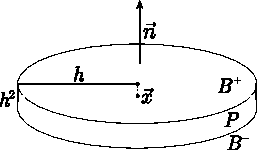
\includegraphics[width=0.6\textwidth]{images/sample.pdf}
% \caption[caption za v kazalo]{Dolg caption pod sliko}
  \caption[Primer vektorske slike.]{Primer vektorske slike z oznakami v enaki pisavi, kot jo
     uporablja \LaTeX{}.  Narejena je s programom Inkscape, \LaTeX{} oznake so importane v
     Inkscape iz pomožnega PDF.}
  \label{fig:sample}
\end{figure}

\begin{figure}[h]
  \centering
  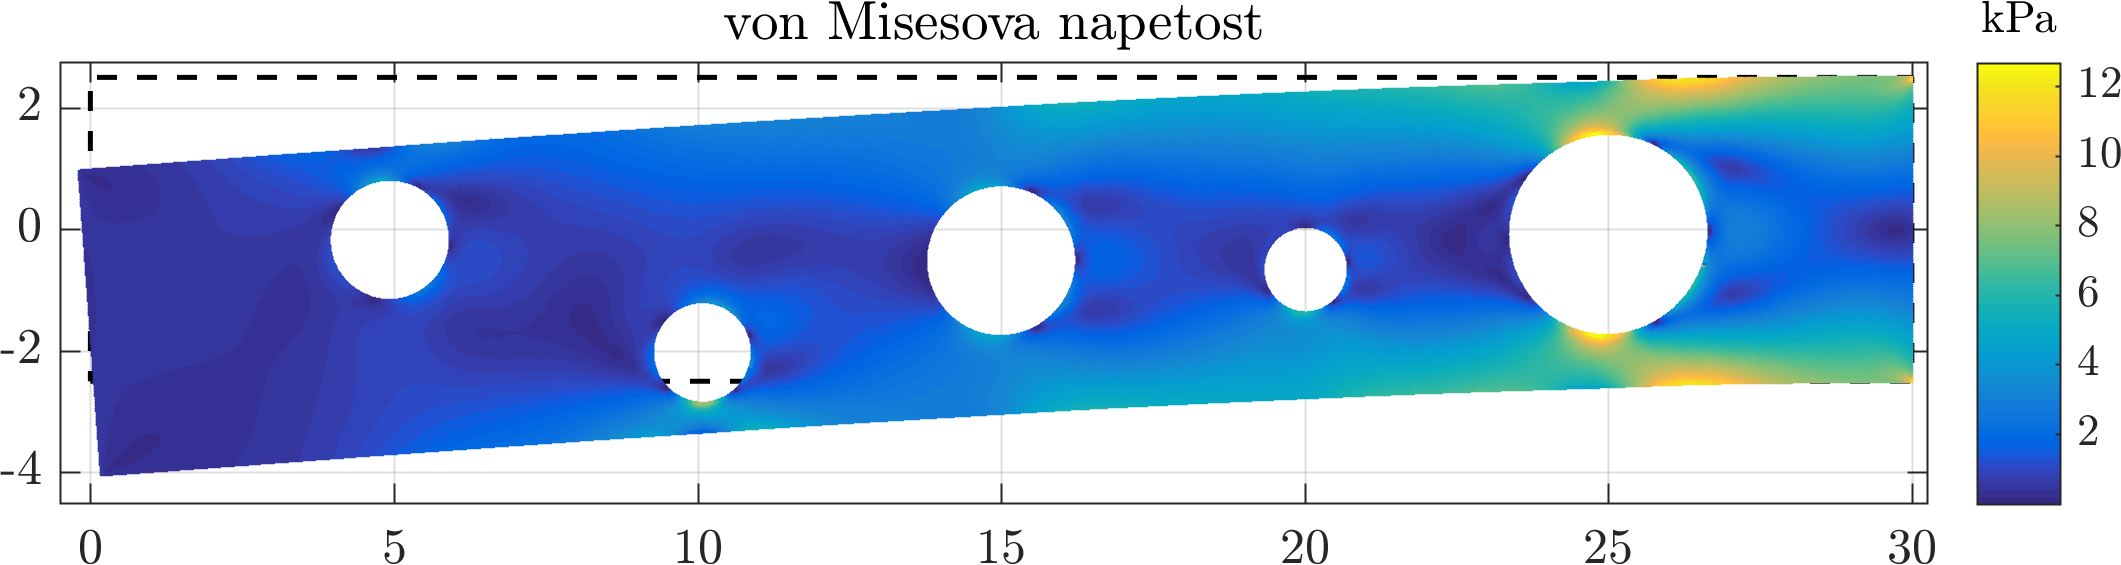
\includegraphics[width=0.8\textwidth]{images/image.png}
  \caption[Primer bitne slike.]{Primer bitne slike, izvožene iz Matlaba. Poskrbite, da so slike v
  dovolj visoki resoluciji in da ne vsebujejo prosojnih elementov (to zahteva PDF/A-1b format).}
  \label{fig:image}
\end{figure}

\subsection{Kako narediti stvarno kazalo}
Dodate ukaze \verb|\index{polje}| na besede, kjer je pojavijo, kot tukaj\index{tukaj}.
Več o stvarnih kazalih je na voljo na \url{https://en.wikibooks.org/wiki/LaTeX/Indexing}.

\subsection{Navajanje literature}
%Članke citiramo z uporabo \verb|\cite{label}|, \verb|\cite[text]{label}| ali pa več naenkrat s
%\verb|\cite\{label1, label2}|. Tudi tukaj predhodno besedo in citat povežemo z nedeljivim presledkom
%$\sim$. Na primer~\cite{chen2006meshless,liu2001point}, ali pa \cite{kibriya2007empirical}, ali pa
%\cite[str.\ 12]{trobec2015parallel}, \cite[enačba (2.3)]{pereira2016convergence}.
%Vnosi iz \verb|.bib| datoteke, ki niso citirani, se ne prikažejo v seznamu literature, zato jih
%tukaj citiram.~\cite{vene2000categorical}, \cite{gregoric2017stopniceni}, \cite{slak2015induktivni},
%\cite{nsphere}, \cite{kearsley1975linearly}, \cite{STtemplate}, \cite{NunbergerTand}.

Tu na novo citiram \cite{DPHclanek1}, \cite{DPHclanek2}, \cite{beltranmonterde}, \cite{choi2002clifford},
\cite{struik1961lectures}, \cite{kreyszig2019differential}, \cite{faroukietal2004}, \cite{farouki2008pythagorean}. 

% Literatura:
% Primer navajanja na http://www.fmf.uni-lj.si/storage/24240/LiteraturaM.pdf,
% ampak bi moral stil poskrbeti za vse. Reference se uredijo po abecedi.
% Če nobena izbira izmed @book, @atricle,... ni ok, potem se lahko vse napiše v
% @misc pod note={} in deluje tako kot normalen LaTeX.
% Komentar v bib datoteki se naredi samo s parom { }
% Za urejanje literature avtor priporoča program Jabref, ki zna tudi avtomatsko
% okrajšati imena revij. Za pravilno sortiranje vnosov brez avtorja, uporabite
% polje key={ }, kot v primeru.
% V primeru napak ustvarite issue na GitHubu ali pišite na jure.slak@fmf.uni-lj.si.
\cleardoublepage                           % na desni strani
\phantomsection                            % da prav delujejo hiperlinki
\addcontentsline{toc}{section}{\bibname}   % dodajmo v kazalo
\bibliographystyle{fmf-sl}                 % uporabljen stil je v datoteki fmf-sl.bst, na voljo tudi angleška verzija
\bibliography{literatura.bib}                 % literatura je v datoteki, definirani na začetku
% TeXStudio zmede \ zgoraj, tako da lahko notri napišeš dejansko ime .bib datoteke, če ti
% ne delajo predlogi citatov.

% Za stvarno kazalo
\cleardoublepage                           % na desni strani
\phantomsection                            % da prav delujejo hiperlinki
\addcontentsline{toc}{section}{\indexname} % dodajmo v kazalo
\printindex

\end{document}
